\documentclass{article}\usepackage{graphicx, color}
%% maxwidth is the original width if it is less than linewidth
%% otherwise use linewidth (to make sure the graphics do not exceed the margin)
\makeatletter
\def\maxwidth{ %
  \ifdim\Gin@nat@width>\linewidth
    \linewidth
  \else
    \Gin@nat@width
  \fi
}
\makeatother

\IfFileExists{upquote.sty}{\usepackage{upquote}}{}
\definecolor{fgcolor}{rgb}{0.2, 0.2, 0.2}
\newcommand{\hlnumber}[1]{\textcolor[rgb]{0,0,0}{#1}}%
\newcommand{\hlfunctioncall}[1]{\textcolor[rgb]{0.501960784313725,0,0.329411764705882}{\textbf{#1}}}%
\newcommand{\hlstring}[1]{\textcolor[rgb]{0.6,0.6,1}{#1}}%
\newcommand{\hlkeyword}[1]{\textcolor[rgb]{0,0,0}{\textbf{#1}}}%
\newcommand{\hlargument}[1]{\textcolor[rgb]{0.690196078431373,0.250980392156863,0.0196078431372549}{#1}}%
\newcommand{\hlcomment}[1]{\textcolor[rgb]{0.180392156862745,0.6,0.341176470588235}{#1}}%
\newcommand{\hlroxygencomment}[1]{\textcolor[rgb]{0.43921568627451,0.47843137254902,0.701960784313725}{#1}}%
\newcommand{\hlformalargs}[1]{\textcolor[rgb]{0.690196078431373,0.250980392156863,0.0196078431372549}{#1}}%
\newcommand{\hleqformalargs}[1]{\textcolor[rgb]{0.690196078431373,0.250980392156863,0.0196078431372549}{#1}}%
\newcommand{\hlassignement}[1]{\textcolor[rgb]{0,0,0}{\textbf{#1}}}%
\newcommand{\hlpackage}[1]{\textcolor[rgb]{0.588235294117647,0.709803921568627,0.145098039215686}{#1}}%
\newcommand{\hlslot}[1]{\textit{#1}}%
\newcommand{\hlsymbol}[1]{\textcolor[rgb]{0,0,0}{#1}}%
\newcommand{\hlprompt}[1]{\textcolor[rgb]{0.2,0.2,0.2}{#1}}%

\usepackage{framed}
\makeatletter
\newenvironment{kframe}{%
 \def\at@end@of@kframe{}%
 \ifinner\ifhmode%
  \def\at@end@of@kframe{\end{minipage}}%
  \begin{minipage}{\columnwidth}%
 \fi\fi%
 \def\FrameCommand##1{\hskip\@totalleftmargin \hskip-\fboxsep
 \colorbox{shadecolor}{##1}\hskip-\fboxsep
     % There is no \\@totalrightmargin, so:
     \hskip-\linewidth \hskip-\@totalleftmargin \hskip\columnwidth}%
 \MakeFramed {\advance\hsize-\width
   \@totalleftmargin\z@ \linewidth\hsize
   \@setminipage}}%
 {\par\unskip\endMakeFramed%
 \at@end@of@kframe}
\makeatother

\definecolor{shadecolor}{rgb}{.97, .97, .97}
\definecolor{messagecolor}{rgb}{0, 0, 0}
\definecolor{warningcolor}{rgb}{1, 0, 1}
\definecolor{errorcolor}{rgb}{1, 0, 0}
\newenvironment{knitrout}{}{} % an empty environment to be redefined in TeX

\usepackage{alltt}
\usepackage{url}
\usepackage{graphicx}
\usepackage{caption}
\title{Global Temperature Anomalies}
\author{Geoffrey Thompson and Sam Benidt}
\date{11/15/2012}
\begin{document}


\maketitle




\section{Introduction}
The consensus of climate scientists is that the world has been warming since the Industrial Revolution and that it has been warming faster over the last several decades. The warming is not uniform - the poles are warming faster than the tropics, for instance. The HADCRUT4 data set has a monthly record of temperature anomalies on a $5^{\circ}$ by $5^{\circ}$ gridded basis going back to 1850, so we can graphically explore when and where temperatures have been changing and by how much over the past 162 years. The HADCRUT4 dataset was the subject of some controversy in October when a journalist claimed the data showed no increase in temperature over the last 16 years.

\section{Description of Data and Source:}
We pulled data on temperature deviations from a 1961 to 1990 temperature trend from the HADCRUT4 near surface temperature data set found at: \url{http://www.metoffice.gov.uk/hadobs/hadcrut4/data/current/download.html}. This data is hosted by the Met Office Hadley Centre. The HADCRUT4 dataset combines data from the  CRUTEM4 and HadSST3 which contain data based on surface air temperature and sea-surface temperature respectively. The data is reported in 100 ensembles. We chose to look at the first ensemble, though the same type of analysis recorded here could be used on any of the 100 ensembles.  The Global temperature trend was also downloaded which is computed from average of the Northern and Southern Hemispheres ((NH +SH)/2).

\section{Data Cleaning/Formatting:}
The temperature deviation data for ensemble 1 was downloaded in a spaced delimited ASCII file.  The ASCII file was opened up in Microsoft Excel and parsed to create a CSV file that contained meta data for the first month of 1850 on the first row followed by 36 rows and 72 columns of temperature deviations where the entry in row i and column j represented a measurement of temperature deviation for each latitude and longitude. This was followed by another row of metadata describing the second month of 1850 following by the same 36 rows by 72 columns of temperature deviations and so on. The CSV file was read into R. Each 37th row was deleted (including the first row) since those rows contained meta data. The variables time (in months since 1850), xloc, months (month of year), year(years since 1850). The data were reshaped to using the melt function keeping the variables time, xloc, months, year, and temp, allowing the yloc variable to be formed.  The variables real year and latitude and longitude were introduced to the data set through an appropriate transformation of the variables $year$, $xloc$, and $yloc$.
Global montly temperature deviation data was downloaded as well. However, there was not much work needed to put the data into a useable format.

\section{Main Section:}
This is still being worked on. There will be some discussion (without modeling) of the overall trend in the data: 
\begin{figure}[h!]
\begin{knitrout}
\definecolor{shadecolor}{rgb}{0.969, 0.969, 0.969}\color{fgcolor}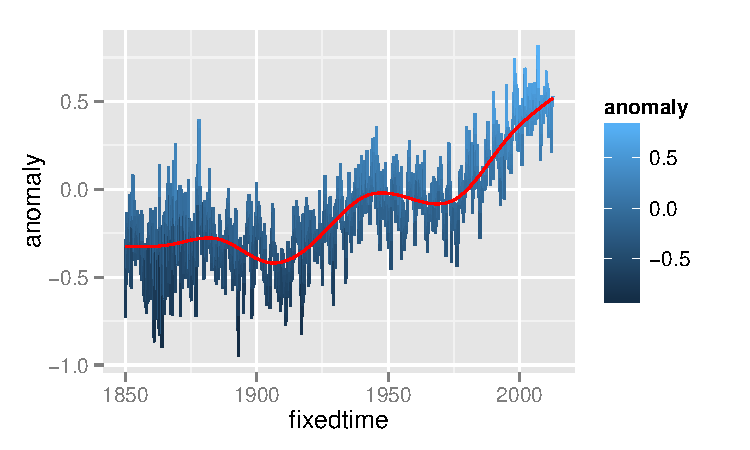
\includegraphics[width=\linewidth]{figure/plot-trend} 
\end{knitrout}

\caption{\label{trend}Time series of global temperature anomalies, 1850-present.}
\end{figure}

There will also be a discussion of what the recent data look like, in light of the "controversy" about the last 16 years of data: 

\begin{figure}[h!]
\begin{knitrout}
\definecolor{shadecolor}{rgb}{0.969, 0.969, 0.969}\color{fgcolor}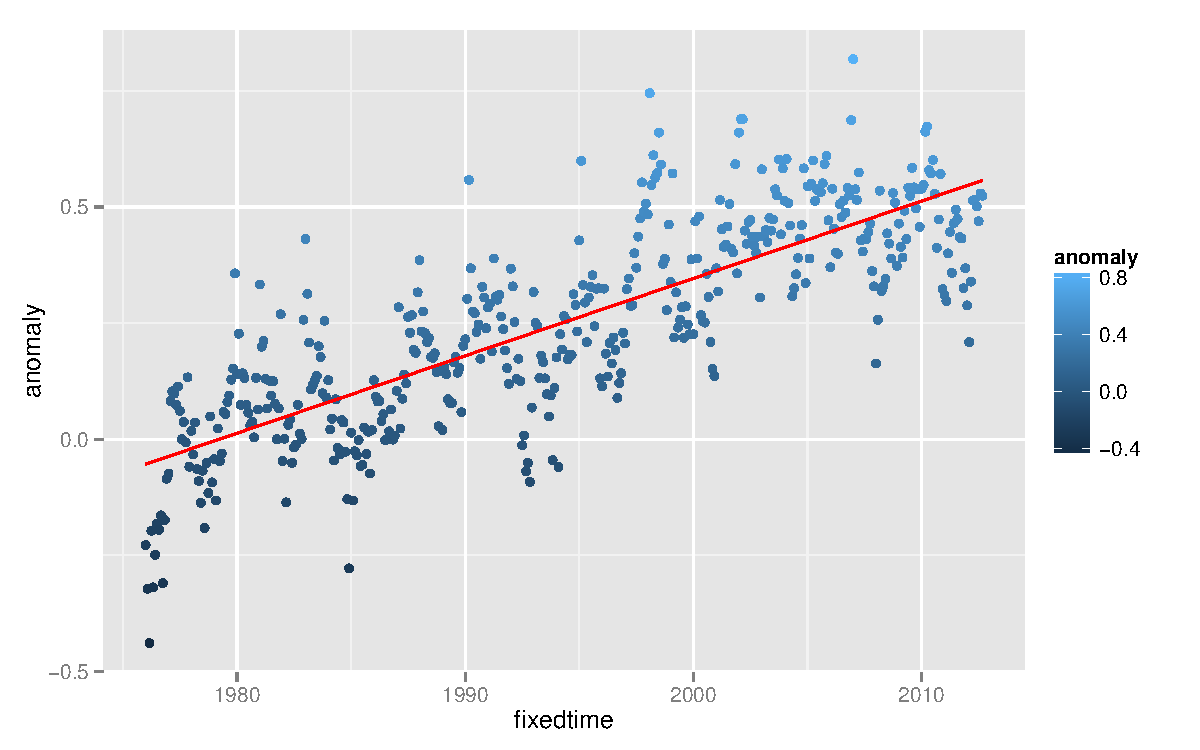
\includegraphics[width=\linewidth]{figure/recent-trend} 
\end{knitrout}


\caption{\label{recenttrend}Time series of global temperature anomalies, 1975-present.}
\end{figure}


There will also be a few maps of some specific time periods. This is the latest map, which shows the difference between the average temperature in September 2012 from the average in 1961-1990. Note that not every grid point has an entry and that not every grid point is greater than 0. 

\begin{figure}[h!]
\begin{knitrout}
\definecolor{shadecolor}{rgb}{0.969, 0.969, 0.969}\color{fgcolor}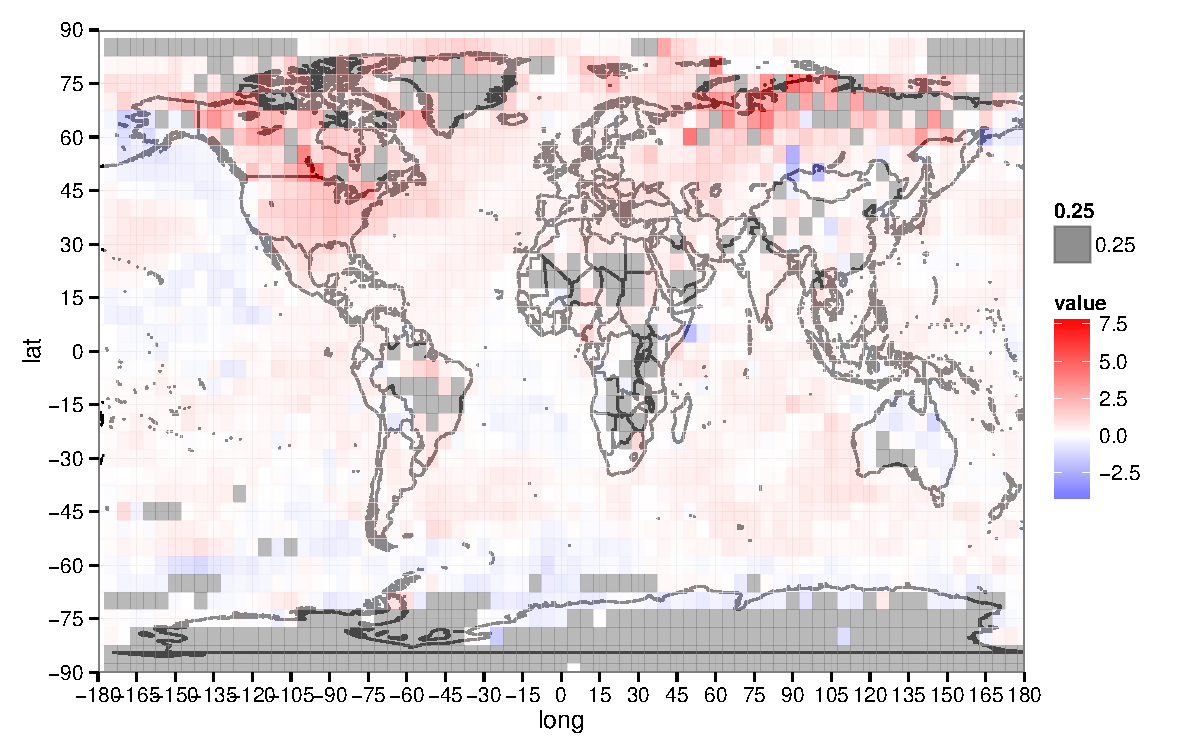
\includegraphics[width=\linewidth]{figure/recent-map} 
\end{knitrout}


\caption{\label{sep2012map}Map of temperature anomalies for September 2012}
\end{figure}



\section{Conclusion:}
There will be some kind of conclusion.
\end{document}
